\documentclass[bachelor,german]{hgbthesis}
\RequirePackage[utf8]{inputenc}
\usepackage{amsmath}
\usepackage{stackengine}
\usepackage{graphicx} 
\usepackage{float}
\bibliography{literatur}  	% name of the BibTeX (.bib) file

\setlength{\parindent}{0pt}
\graphicspath{{images/}}
\begin{document}

\title{Klassifikation und Clustering}
\author{Krainer Philipp}
\studiengang{Medizin- und Bioinformatik}
\studienort{Hagenberg}
\abgabedatum{2016}{05}{30}	% {YYYY}{MM}{DD}

\nummer{1310458007-A}   % XX...X = Stud-ID, z.B. 0310238045-A  
												%%% (A = 1. Bachelorarbeit)
\gegenstand{Softwareentwicklung mit klassischen Sprachen}                      
\semester{Sommersemester 2015} 
\betreuer{Stephan Winkler}


\frontmatter
\maketitle


%
\tableofcontents
%
%
\chapter{Kurzfassung}
Die vorliegende Arbeit setzt sich mit den heuristischen Algorithmen der Klassifikation und  des Clustering auseinander. \\ Das Clustering, welches auch als unüberwachte Klassifikation bekannt ist, wird als eine Methode zur Einteilung von großen Datensätzen angewandt. Hier wird auf den unterschiedlichen Bezug der Daten  auf das Clustering und dessen Algorithmen eingegangen. Verschiedene Algorithmen geben einen guten Einblick in die komplexe Welt des Clustering. Grundsätzlich gilt, dass jede Methode ihr eigenes Einsatzgebiet innehat und an die vorliegenden Daten anzupassen ist.\\ 
In weiterer Folge wird mit der Klassifikation eine weitere Methode beschrieben Daten einzuteilen. Im Gegensatz zum Clustering werden bei Klassifikation Daten anhand vorgegebener Klassen zugeordnet. \\
Auch hier wurden die verschieden Algorithmen unter der Berücksichtigung der Klassifikationsgüte beschrieben und verglichen. Alle Algorithmen verwenden bereits vordefinierte Daten und Methoden um die Berechnung zu beschleunigen. Daher ist die Klassifikation weiterverbreiteter als das Clustering. \\ Es wurden die Algorithmen und Methoden anhand von  Beispielen  entsprechend dargestellt. Dabei kamen das Heuristiclabtool sowie Daten aus UCI Repository zur Anwendung. Diese Beispiele zeigen ziemlich gut welche Algorithmen für welche Datensätze geeignet sind und beste Ergebnisse liefern.

\begin{english}
\chapter{Abstract}
This thesis deals with the comparison of heuristic algorithms of classification and clustering.\\
First we discuss clustering as a part of the unsupervised classification. This is used to divide big data into smaller and different parts.
Different algorithms and Methods describe the common used strategies of clustering relatively well. Basically every data set is different and not every algorithm can be applied to it, so every method has to be customized to fit into the data set properties.\\
In contrast to the Clustering the Classification separates data sets based on predefined classes in groups by using train data and test data. 
Different algorithms are described to show a number of different methods to use classification. 
A main measurement for the algorithms is basically classification quality. 
All algorithms use predefined data to boost computing performance. That means Classification is used more often than clustering. Finally some examples and tests of the different algorithms of classification and clustering are described.\\
The HeuristicLab software is used for the calculation of the algorithms and the sample data is provided from the UCI repository. All samples show us which kind of algorithms can be used for the different data sets and the best results.
\end{english}
\mainmatter
\chapter{Einleitung}\label{Einleitung}
\section{Einführung}
In dieser Bachelorarbeit werden die Themen \emph{Klassifikation} und \emph{Clustering} in Bezug auf heuristische Methoden behandelt. In der heutigen Welt sind große Datenmengen an der Tagesordnung. Die Hardware ist zwar leistungsfähig genug, kann aber große Datensätze nicht auf einmal verarbeiten, da die zeitliche Datendurchsatzrate zu gering ist. Daher ist es entscheidend große Datenmengen in kleinere Einheiten mit Hilfe von Klassifikation und Clustering überzuführen. Der Begriff \textit{Big Data} bestimmt die Welt der Analyse und der Verarbeitung von Informationen, welche meist als mehrdimensionale Daten beschrieben werden können. Daher ist es wichtig geeignete Algorithmen und Verfahren zu finden, welche große Datenmengen in anwendbare Einheiten einteilen.\\Das Ziel der Analyse von eingeteilten Daten ist es eine verständliche und interpretierbare Konzeption zu erreichen, welche auf einem geeigneten Modell basiert. Dieses Modell kann nur auf der Basis von eingeteilten Daten funktionieren, da es sonst zu komplex wird. Das Clustering und die Klassifikation machen diese Vorgangsweise erst möglich. Sie sind daher ein zentraler Bestandteil bei der Analyse von Daten und in der Heuristik und in der Statistik nicht mehr wegzudenken.  
\section{Aufgabenstellung}
In der Klassifikation geht es darum Samples in verschiedene Klassen einzuteilen. Beim Clustering dagegen geht es darum Gruppen von Datenpunkten zu identifizieren. Ist es sinnvoll Daten vor dem Anwenden von Klassifikationsalgorithmen zu gruppieren, also Clustering und Klassifikation zu kombinieren. Lässt sich so die Prognosegenauigkeit erhöhen? Ziel dieser Arbeit ist es, Antworten auf diese Fragen zu finden; Frameworks wie das HeuristicLab und WEKA sowie international bekannte Benchmark-Datensätze können für die entsprechenden Tests verwendet werden.


\section{Terminologien und Begrifflichkeiten}
\begin{itemize}
	\item \textbf{Heuristik:}\\ Aus dem Griechischen heuriskein = finden, entdecken, bezeichnet eine Erfinderkunst. Heuristik ist die Lehre von verschiedenen Verfahren zum Lösen von Problemen, welche nicht mit mathematischen Algorithmen bzw. Formeln gelöst werden können.
\item \textbf{Datensatz:}\\ Ein Datensatz ist die Zusammenfassung von Daten, die in einer direkten Beziehung zueinander stehen oder gemeinsame Merkmale haben. Daten, die in einem Sinnzusammenhang stehen, können dabei in einem Ordnungssystem zusammengefasst sein.
\item \textbf{Wahrscheinlichkeit:}\\ Die Wahrscheinlichkeit ist ein Maß zur Quantifizierung der Sicherheit bzw. Unsicherheit des Eintretens eines bestimmten Ereignisses im Rahmen eines Zufallsexperiments
\item \textbf{Algorithmus:}\\Ein Algorithmus ist eine eindeutige, ausführbare Folge von Anweisungen endlicher Länge zur Lösung eines Problems. Ein Algorithmus besteht aus einem Deklarationsteil und einem Anweisungsteil.
\item \textbf{Sample (Sampling):}\\Teilmenge einer Grundgesamtheit, die für eine Untersuchung ausgewählt wird.
\item \textbf{Satz von Bayes:}\\Der Satz von Bayes ist ein mathematischer Satz aus der Wahrscheinlichkeitstheorie, der die Berechnung bedingter Wahrscheinlichkeiten beschreibt. Formel: \[P(A|B)=\frac{P(A)\cdot P(B|A)}{P(B)}=\frac{P(A\cap B)}{P(B)}\]
\item \textbf{Test:}\\ Tests sind Methoden, mit denen eine Entscheidung über die Beibehaltung oder Zurückweisung einer Nullhypothese \(H_0\) mithilfe eines Stichprobenbefundes getroffen wird.
\item \textbf{Graph:}\\Ein Graph ist in der Graphentheorie eine abstrakte Struktur, die eine Menge von Objekten zusammen mit den zwischen diesen Objekten bestehenden Verbindungen repräsentiert. Die mathematischen Abstraktionen der Objekte werden dabei Knoten des Graphen genannt. Die paarweisen Verbindungen zwischen Knoten stellen Kanten dar.
\item \textbf{Daten:}
	\begin{itemize}
		\item numerisch:\\Daten, die  mit Ziffern und zusätzlichen Sonderzeichen dargestellt werden.
		\item nicht-numerisch:\\Daten, die aus Buchstaben und Ziffern zusammengesetzt sind.
	\end{itemize}
	\item \textbf{Zeitreihe:}\\Ein Zeitreihe ist eine Serie von Messungen, Beobachtungen und Aufzeichnungen von Variablen an aufeinanderfolgenden Zeitpunkten. Zeitreihen ermöglichen eine strukturierte Darstellung von Daten. Eine visuelle Darstellung entspricht einer Kurve, die sich mit der Zeit entwickelt.
	\item \textbf{Dimension:}\\  Der Begriff Dimension bezeichnet im Allgemeinen lediglich ein unabhängiges Merkmal eines Datensatzes. Dimensionen haben mit den Daten selbst gar keine echte Verwandtschaft, sondern stellen meist ein unabhängiges Gedankenkonstrukt dar, das Analogien zum Datensatz herstellt, um es berechenbar oder messbar zu machen.
\item \textbf{Distanzmaß:}\\ Als Distanzmaß wird ein Maß bezeichnet, wenn es die Unähnlichkeit zwischen zwei Objekten misst. Es besitzt die Eigenschaft, dass es mit zunehmender Unterschiedlichkeit zweier Objekte ansteigt.
\item \textbf{Kostenfunktion:}\\ Als Kostenfunktion wird jene Funktion beschrieben, welche bestimmt wie komplex und aufwendig ein Algorithmus oder Verfahren ist. Meist wird diese Funktion mit der O-Notation gleich gesetzt, welche vor allen in der Laufzeitmessung angewandt wird.
\item \textbf{Lagemaße:}
	\begin{itemize}
		\item Mittelwert:\\ Der Mittelwert beschreibt den statistischen Durchschnittswert und wird auch arithmetisches Mittel genannt. 
		\item Median:\\Der Wert, der genau in der Mitte einer Datenverteilung liegt, nennt sich Median oder Zentralwert. Die eine Hälfte aller Daten ist immer kleiner, die andere größer als der Median. 
		\item Modus:\\Der Modus gibt an, welche Merkmalsausprägung in einem Datensatz am häufigsten vorkommt. 
\end{itemize}
\item \textbf{Heatmap:}\\
Eine Heatmap  ist ein Diagramm zur Visualisierung von Daten, deren abhängige Werte einer zweidimensionalen Definitionsmenge als Farben repräsentiert werden. Sie dient dazu, in einer großen Datenmenge intuitiv und schnell besonders markante Werte zu erfassen.
\begin{figure}[H]
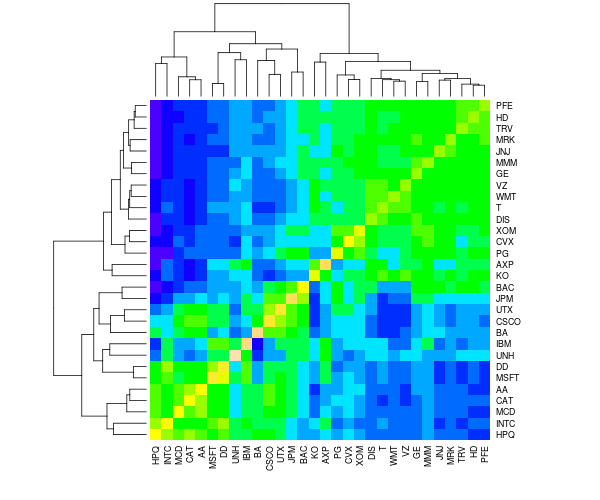
\includegraphics[width=\textwidth]{Heatmap.png}
\caption{heatmap}
\label{}
\end{figure}
\item \textbf{Cluster:}\\
Als Cluster bezeichnet man in der Informatik und Statistik eine Gruppe von Datenobjekten mit ähnlichen Eigenschaften.
\item \textbf{Link Arten:}
\begin{itemize}
		\item Single-Link:\\ Beschreibt die kleinste Entfernung von den Clustern und wird auch als nächster Nachbar bezeichnet.
		\item Average-Link:\\Beschreibt die mittlere Distanz von Clustern zueinander
		\item Complete-Link:\\ Beschreibt die maximale Entfernung von Clustern zueinander.
\end{itemize}
\end{itemize}

\chapter{Clustering}\label{Clustering}
\section{Einführung}
In der Informatik und Statistik sind große Datensätze anzutreffen. Diese können analysiert werden, wenn entsprechende Tools und Algorithmen zur Verfügung stehen. Durch das Verfahren von Clustering und Bildung von eingeteilten Datensätzen wird das Arbeiten mit großen Daten erleichtert. Das Ziel ist ein geeignetes Modell für einen gegeben Datensatz zu finden. Durch diese Methoden wird das Interpretieren von Merkmalen und Besonderheiten erleichtert und ermöglicht außerdem eine begünstigte Aufbereitung von den Daten.\cite{fasulo99}\\Um die richtigen Modellrepräsentationen  zu finden und diese zu identifizieren ist es notwendig die Daten zuerst in Klassen einzuteilen. Damit beschäftigt sich die \nameref{Klassifikation}. Dies ist sehr hilfreich wenn ein klassenorientiertes Clustering vorgenommen wird, da die Einteilung zu relevanten Merkmalen zuerst erfolgen muss.
Dabei wird zwischen zwei Arten unterschieden: Die überwachte (\textit{supervised}) und die unüberwachte(\textit{unsupervised}) Klassifikation.\cite{fasulo99} \\
Clustering gehört zu der unüberwachten Klassifikation, welche die Daten in relevante Klassen sogenannte Cluster einteilt. \\
Das Einsatzgebiet von Clustering-Algorithmen ist vielfältig. Die Anwendungsgebiete sind vor allem im Gebiet von Data-Mining und Data-Analysis zu finden. Weitere Anwendungsgebiete sind die Bioinformatik, Analyse von Datenbanken, Textmining u. Neuronale Netzwerke. Clustering spielt bei der Datenanalyse eine große und bedeutende Rolle.\cite{fasulo99} 



\section{Datenrepräsentation}
Als \textsl{Daten} wird eine Ansammlung bzw. eine Menge an Dingen oder Objekten bezeichnet. Diese Definition bezieht sich auf den Zusammenhang von Daten und Clustering. Jedes einzelne Objekt besitzt spezielle Eigenschaften, welche eindeutig per Objekttyp sein können. Diese Eigenschaften werden oft auch als Attribute, Merkmale oder Dimensionen bezeichnet.\cite{pell91}\\In einen Datenraum befinden sich Objekte oder Elemente mit einer endlichen Anzahl von Merkmalen, welche bei allen Objekten denen des Datenraumes gleichen. Jedoch können sich Daten die sich innerhalb dieses vorgegebenen Raumes befinden sich unterscheiden, da die Ausprägung nicht vorgegeben ist. \cite{pell91}
Dabei gibt es eine mathematische Repräsentation:\\


\noindent\(D,D_d:\) Datenraum (auch Merkmalsraum) der Dimension \textit{d} (auch \(\mathbb{R}^d\))\\

\noindent\(S:\) Datenmenge, \(S \subset D \)\\

\noindent\(x_i:\) \textsl{i}-tes Objekt aus \(S\)\\

\noindent\(|S|,n:\) Mächtigkeit von S (Anzahl von Objekten)\\[5px]

\def\tmp{%
\begin{matrix}
  x_1= &(  x_{1,1} & \cdots & a_{1,d} ) \\
 x_2 = & (  x_{2,1} & \cdots & a_{2,d} ) \\
\vdots &   \vdots  & \ddots & \vdots  \\
 x_n & ( x_{n,1} & \cdots & a_{n,d}  )


\end{matrix}
}%
\[  
\stackMath\def\stackalignment{r}%
  \stackon%
    {\mathrm{\text{Objekte}}\left\{\tmp\right.}%
    {\overbrace{\phantom{\smash{\tmp\mkern -82mu}}}^{\mathrm{\textstyle Attribute}}\mkern 15mu}
\]\\[5px]

Jedes einzelne Objekt aus der Datenmenge \textsl{S} hat \textsl{d} Merkmale/Attribute. Diese werden durch die Art (des Typs) unterschieden. Dabei wird zwischen \textit{numerisch} und \textit{nicht-numerisch} Daten unterschieden. \\

Erstens betroffen sind die Daten bzw. Objekte in Vektoren von reelwertigen Zahlen. Als Beispiel sei eine Zeitreihe von einer Messung genannt.  Zweitens betrifft den Rest, welcher in ein numerisches Format übertragen werden kann. Im Allgemeinen können \textit{nicht-numerische} Merkmale durch spezifische Codierungen in numerische Merkmale übertragen werden. Dabei wird jedes einzelne Merkmal durch ein oder mehrere Attribute repräsentativ dargestellt.\cite{pell91}\\ 
Diese Methode wird verwendet um \textit{numerische} und \textit{nicht-numerische} Daten gleich zu behandeln, da es dabei keinen Unterschied in der Anwendung bzw. Auswertung gibt. Diese Methode ist notwendig um die Daten in ein Format zu bringen, welches für das Clustering verwendet werden kann. Dann können die Daten von einem geeigneten Algorithmus verarbeitet werden.\cite{pell91}\\ 
Doch in der realen Welt sind große und komplexe Daten an der Tagesordnung. Doch im Gegensatz dazu würde es sich sehr aufwändig gestalten, wenn  Algorithmen mit hoher Dimensionalität an Daten verwendet werden. Da sich dabei die Rechenzeit erheblich erhöhen würde müssen Methoden angewendet werden um die Datenkomplexität zu reduzieren. Bei vielen Datensätzen sind  zu viele Merkmale vorhanden, die sogar irrelevant für die Berechnung sind. Manche können den Algorithmus sogar in eine falsche Richtung führen.\cite{pell91}\\
Einerseits gibt es die Möglichkeit gewisse Merkmale auszuklammern d.h. diese werden nicht in die Berechnung aufgenommen um die Komplexität zu verringern. Dabei gehen keine wichtigen Attribute verloren. Dieses Verfahren wird als Merkmalsauswahl(\textit{featuren selection}) genannt. Es ist oft hilfreich nur gewisse Merkmale auszuwählen, um eine Selektion von den Besten zu ermöglichen (auch Elitismus genannt), denn dann sind die Algorithmen performant und liefern annehmbare Ergebnisse.\cite{pell91}\\ 
Eine weitere Möglichkeit ist es gewisse Merkmale aus einer Ansammlung auszuwählen. Dadurch kann auch eine Featurereduktion erreicht werden. Dies ist ebenso so effizient wie die Auswahl der Merkmale.  Diese Methode wird Merkmalsextraktion(\textit{feature extraction}) genannt. Dabei werden nur die wichtigsten Merkmale herangezogen, um die Performance zu steigern.\cite{pell91}\\
Neben den beiden Methoden ist es auch notwendig die Daten zu normalisieren d.h es müssen die Daten auf die gleiche Weise umgerechnet werden, damit sie besser zusammenpassen. Dies wird durch skalieren und konvertieren erreicht.  Die Normalverteilung der Daten wird angenommen um die Skalierung zu erleichtern; mit denselben Mittelwert (\(\bar{x}\)) und der selben Standardabweichung (\(\sigma\)), mit \(\bar{x} = 0\) und \(\sigma = 1\).\cite{pell91}\\
Bevor die Algorithmen angewendet werden können, muss ein geeignetes Maß für den Abstand gefunden werden.  Die Maße sind metrisch u. es wird daher der Überbegriff der Ähnlichkeitsbestimmung verwendet. Diese Maße geben an wie ähnlich sich zwei Objekte sind und  dabei wird nicht zwischen \textit{numerisch} und \textit{nicht-numerisch} unterschieden. Das Distanzmaß (\textit{distance measure}) oder Ähnlichkeitsmaß(\textit{similarity/proximity/affinity measure}) definiert die Beziehung bzw. die Funktion \(d: D \times D \rightarrow Z \). Die Maße sind essentiell für das Clustering und müssen vor den eigentlichen Clustering ausgeführt werden.\cite{fasulo99}

\section{Algorithmen}

\subsection{Allgemein}
Nachdem ein geeignetes Distanzmaß gefunden ist, kann ein bestimmter Algorithmus auf die Daten angewendet werden. Es gibt zwei Gruppen von Verfahren bzw. Algorithmen, welche das  \textit{Hierarchisches Clustering} und die \textit{Partitionierung} darstellen. Bei der Partitionierung werden die Objekte bzw. Daten in Gruppen eingeteilt und diese Gruppen enthalten keine weiteren verschachtelten Cluster und besitzen nur eine Ebene. Beim \textit{Hierarchischen Clustering} entsteht ein geschachtelter Aufbau bzw. eine Struktur, wo größere Cluster kleinere enthalten.\cite{fasulo99}\\

Weiters können die beiden oben angeführten Methoden weiter aufgegliedert werden:\cite{fasulo99}

\begin{itemize}
	\item\textit{divisiv:}\\
	Bei dieser Methode werden alle Objekte einen Cluster zugeordnet sowie schrittweise verkleinert, indem schrittweise zerteilt wird, bis ein vordefiniertes Abbruchkriterium eintritt.\\
	
	\item\textit{agglomerativ:}\\
	Im Gegensatz zu der divisiven Methode wird bei der agglomerativen Methode mit kleinen Clustern begonnen. Jedes Objekt stellt einen Cluster für sich dar. Die kleinen Cluster werden schrittweise zusammengefügt bis ein Abbruchkriterium eintritt.\\
	
	\item\textit{hard:}\\
	Algorithmen welche das Prinzip von einer strikten Vorgehensweise (\textit{hard}) verfolgen ordnen einen Cluster ein Objekt zu.\\
	
	\item\textit{fuzzy:}\\
	Im Gegenteil dazu gibt es das Prinzip von der ungenauen Vorgehensweise(\textit{fuzzy}), dabei können Objekte verschiedenen Clustern zugeordnet werden. \\
	
	\item\textit{stochastisch:}\\
		Bei dem Begriff stochastisch kann davon ausgegangen werden, dass der Zufall eine Rolle spielt und die Auswahl verschiedener Objekte oder Attribute keiner Regel folgt.\\
	
	
	\item\textit{deterministisch:}\\
	Dabei handelt es sich um die Vorgabe keiner zufälligen Ereignisse. Hier muss alles vorgegeben sein damit es als deterministisch gilt.\\
	
	\item\textit{monothetisch:}\\
	Wenn bei der Verarbeitung nur ein Cluster bzw. ein Objekt verarbeitet wird, dann wird dieses Verfahren monothetisch bezeichnet. Aber die Algorithmen arbeiten nur bedingt nach diesem Prinzip, da dadurch die Berechnungszeit erhöht sein kann.\\
	
		\item\textit{polythetisch:}\\
		Bei der polythetischen Vorgangsweise werden Cluster bzw. Objekte oder Daten schneller verarbeitet, da Vorgänge gleichzeitig ausgeführt werden. In Bezug auf das Clustering bezieht sich die Gleichzeitigkeit auf die Distanzberechnung der Merkmale. 
	
\end{itemize}

\subsection{k-means Algorithmus}
\subsubsection{Beschreibung:}
Der \textit{k-means} Algorithmus gehört zu den Partitionierungs-Algorithmen. Die Implementierung ist einfach und liefert trotzdem gut interpretierbare Ergebnisse für einfache Aufgabenstellungen. Grundlegend versucht der Algorithmus eine Partition in den Daten zu finden und daraus dann Cluster zu bilden. Die Anzahl der Cluster wird durch den Anwender festgelegt und während der Laufzeit nicht mehr geändert. Die Formel nach dem die Cluster gebildet werden lautet: \cite{pell91} \\

\[x_r^i: r\textrm{-te Element des Clusters}\ C_i\]
Diese Methode wird auch als Sum-of-Squares bezeichnet. Dabei werden die quadratischen Abstände minimiert. Beim Clustering bedeutet dies, dass die Ähnlichkeit der Attribute, Merkmale oder Objekte bestimmt wird. Damit basieren Cluster auf der oben angeführten Kostenfunktion.

\subsubsection{Algorithmus:}
\begin{enumerate}
\item Wähle zufällig \(k\) Cluster-Zentren \(\mu_1,\dotsc,\mu_k\).\\


\item Berechne für jedes \(x \in S\), zu welchen Clustermittelpunkt \(\mu_i\) es am nächsten liegt.\\


\item Berechne für jeden Cluster \(C_i\) die Kostenfunktion:\\
\[c(C_i) = \displaystyle\sum_{r=1}^{|C_i|}(d(\mu_i,x_r^i))^2\]\\

\item Berechne für jeden Cluster \(C_i\) den eigenen neuen Mittelpunk:\\
\[ \mu_i =\frac{1}{|C_i|} \displaystyle\sum_{r=1}^{|C_i|}x_r^i\]\\

\item Wiederhole 2., 3., 4. bis sich die Clusterzuordnung nicht mehr ändert.\\




\end{enumerate}

Die Datensätze besitzen einen Mittelwert, da diese \textit{numerisch} sind. Daher kann ein Mittelwert oder auch das arithmetisches bzw. geometrisches Mittel gebildet werden. Auch beim Clustering können \textit{nicht-numerische} Datensätze verwendet werden. Diese besitzen meistens keinen numerischen Mittelwert.\\

Dennoch kann ein Lagemaß berechnet werden: der Median. Dieser gibt ähnlich wie der Mittelwert eine gute Aussage wie die Daten verteilt sind und es können auch damit \textit{nicht-numerischen} Daten berechnet werden. Beim Clustering wird der ähnliche \textit{k-medioids} Algorithmus angewandt, welcher  nach dem oben genannten Prinzip funktioniert. Nur wird bei der Berechnung der Mittelwert \(\mu\) durch den Median ersetzt. \cite{pell91}

\subsubsection{Zusammenfassung}
Dieser Clusteringalgorithmus ist einfach in seiner Komplexität, da er sich nur auf die Mittelwerte der einzelnen Attribute bezieht. Doch bei der Bildung von Clustern können einfach sphärische Cluster entstehen, da die Berechnung relativ zum Mittelwert geschieht. Weiteres kann ein vorhandenes Rauschen in den Daten (Störung in den Daten) bei diesem Algorithmus nicht beseitigt werden, da der Mittelwert sehr ausreißerempfindlich ist.


\subsection{Hierarchisch Clustering}
\subsubsection{Beschreibung:}
Diese Methode wird verwendet wenn die Daten nicht offensichtlich in Gruppen bzw. Partitionen eingeteilt sind oder es keine separierte Cluster gibt. Diese Methode erstellt eine hierarchische Baumstruktur der Datenmenge. Dabei sind die einzelnen Knoten bzw. Enden jeweils eine Teilmenge des übergeordneten Knotens. Der Wurzelknoten repräsentiert die gesamte Menge und die Blätter die einzelnen Objekte.\\

Bei diesem Algorithmus werden \textit{bottom-up} und \textit{top-down} als Verfahren unterschieden\\

Bei der \textit{bottom-up} Methode wird anfangs von kleinen Elementen bzw. Clustern ausgegangen. Diese werden immer weiter kombiniert bis ein gemeinsamer Megacluster entsteht, welcher den ganzen Datensatz enthält. Wenn ein großer Cluster entstanden ist, ist der Algorithmus durchlaufen bzw. das Clustering abgeschlossen.\cite{jain99, mitch97}\\

Im Gegensatz dazu wird bei der \textit{top-down} Methode von einen einzelnen Cluster ausgegangen, welcher den ganzen Datensatz enthält. Hier wird schrittweise der übergeordnete Cluster, auch \textit{parent} genannt in mehrere kleinere Cluster (\textit{child})zerlegt. Diese stellen den Eltern-Cluster dar. Wenn in jeden Cluster nur mehr ein Element vorhanden ist, ist das Clustering abgeschlossen.\\

Beide Methoden verwenden eine Baumstruktur im Hintergrund, in der die einzelnen Cluster als Knoten repräsentiert werden. Dadurch kann mit größeren und komplexeren Datensätzen gearbeitet werden. \cite{jain99, mitch97}

\subsubsection{Algorithmus}

Der Algorithmus wird anhand der der \textit{bottom-up} Methode erklärt. Dabei wird eine Vereinigung von zwei Clustern verwendet. Die zweite Methode \textit{top-down} kann durch durch teilen der Cluster beschrieben werden:\\

\begin{enumerate}
	\item Beginne mit \(n\) Clustern \(C_1,\dotsc,C_n\); wobei \(C_i = x_i\).\\
	
	\item Minimiere die Kostenfunktion \(c(C_i,C_j)\), um die \textsl{beste} bzw. \textsl{günstigste} Vereinigung ( \(C_i \cup C_j\)) zu finden.\\
	
	\item Ersetze \(C_i\) und \(C_j\) durch die Vereinigung \(C_i \cup C_j\).\\
	
	\item Wiederhole die Schritte 2 und 3 bis alle Cluster zusammengefasst sind. \\
	

\end{enumerate}


Das hierarchische Clustering ist nur ein Verfahren, dass einzelne Algorithmen implementiert. Die Vorgehensweise  unterscheidet sich nur in der Ausführung des Verfahrens. Es wird unterschieden zwischen \textit{Single-Link}, \textit{Average-Link} und \textit{Complete-Link}. Dabei unterscheiden sich die Verfahren nur in der Kostenfunktion:\\

\begin{itemize}
	\item \textit{Single-Link}:\\
	\[c(C_i,C_j) = \min\limits_{x \in C_i, y \in C_j} d(x,y)\]
		\item \textit{Average-Link}:\\
		\[c(C_i,C_j) = \frac{1}{|C_i||C_j|}\displaystyle\sum_{x \in C_i} \displaystyle\sum_{y \in C_j} d(x,y)\]
		\item \textit{Complete-Link}:\\
		\[c(C_i,C_j) = \max\limits_{x \in C_i, y \in C_j} d(x,y)\]\\
\end{itemize}

\cite{fasulo99, jain99, mitch97}
   
\subsubsection{Zusammenfassung}
Die Datenmatrix bzw. der Datenvektor spielen bei dieser Methodik eine geringe Rolle, da eigentlich beim Clustering speziell beim hierarchischen meistens auf die Distanzen Rücksicht genommen wird und diese als Eingabe eingesetzt werden. Meist werden diese Distanzen durch eine Matrix repräsentiert.  Die Dimensionen werden als \(n \times n\) dargestellt, welche bei großen Datenmengen oder großen \(n\) zu Speicherproblemen führen können, da die Datenmenge sehr schnell ansteigen kann. \\
Abhilfe kann geschaffen werden, indem ein Schwellenwert festgelegt wird. Damit werden unbedeutende Wertepaare vernachlässigt. Weiters können auch die Anzahl der verwendeten Elemente begrenzt werden und dadurch die repräsentative Menge der Elemente reduziert werden. Auch können die Verlinkungen zu Nachbarn begrenzt werden um die Anzahl der nächsten Nachbarn zu begrenzen. \\


\subsection{Self-organizing Maps}
\subsubsection{Beschreibung:}
Bei diesen Clusteringverfahren wird ein mehrdimensionaler Datensatz mit einer bestimmten Dimensionalität auf ein Gitter mit wenig Dimensionalität meist ein - oder zweidimensional projiziert. Die Anzahl der Cluster ist festgelegt und kann durch die Spalten und Zeilen im Gitter festgelegt werden. Die Referenzvektoren werden beim SOM Clustering aus den Knoten im Gitter gebildet und durch eine iterative Annäherung anhand des vorgegeben Algorithmus zu den Eingabevektoren geleitet.   \cite{tam99}
\subsubsection{Algorithmus:}

\begin{enumerate}
	\item Wähle ein Gitter mit \(k = k_v \times k_h\) Knoten \(v,v \in \{1,\dotsc,k\}\).\\
	
	\item Initialisiere \(k\) \(d\)-dimensionale Vektoren \(f_0(v)\), durch zufällige Wahl von Objekten \(x \in S\) oder vollständig zufällig\\
	
	\item Iteration \(i\):
	\begin{enumerate}
		\item Für jedes Objekt \(x \in S\) bestimme den Knoten \(v_x\), für den \(f_i(v_x)\) am nächsten zu \(x\) liegt.\\
		
		\item Aktualisiere alle Referenzvektoren wie folgt:\\
		
		\[f_{i+1} = f_i(v) + \eta(d(v,_x),i) \cdot (x - f_i(v)) \]\\
		
		\(\eta(d,i)\): Lernrate; Die Lernrate nimmt mit der Distanz zwischen den Knoten und der Iteration ab.\\
		\item Wiederhole (a) und (b) bis keine Veränderung mehr eintritt.\\
	\end{enumerate} 
\end{enumerate}
\cite{tam99}
\subsubsection{Zusammenfassung}
Bei dem SOM-Algorithmus ist die Reduktion der Dimensionalität an erster Stelle und kann somit sehr effizient zum Berechnen von großen Datensätzen herangezogen werden, da die Dimensionalität bzw. die Anzahl der Merkmale gering ist. Auch eignet sich der Algorithmus um Daten aufzuteilen, da die Clusteranzahl vorbestimmt ist und so ein vereinfachter Algorithmus angewendet werden kann. 

\subsection{Graph-based Clustering}
Beim \textit{Graph-based Clustering} wird von einem Graphen ausgegangen, welcher die Distanzmatrix repräsentiert. Die Knoten im Graphen werden Objekten aus der Datenmenge zugeordnet. Die verbindenden Linien oder auch Kanten entsprechen der Distanz zwischen den einzelnen Objekten. Diese können \textit{gerichtet} oder \textit{ungerichtet} sein.\cite{fasulo99,jain99} \\
Das Verfahren versucht den Graphen zu zerteilen und ist auch in der Heuristik als Graphpartionsproblem bekannt. Meistens wird eine rekursive Bipartitionierung angenommen, da diese sehr effizient zu berechnen ist. Dabei sind die Graphen eine repräsentative Darstellung von Ähnlichkeitsbeziehungen der einzelnen Objekte.\cite{jain99}\\
Eine weit verbreitete Methode bei Clustering mit Hilfe von Graphen wird \textit{Clique-based Clustering} genannt. Dabei wird durch die Cliquengraphen die Beziehungen zwischen Objekten und deren Ähnlichkeit gezeigt. Im Idealfall sind die Objekte in einen Cluster sehr ähnlich zueinander und die Objekte die zu anderen Clustern gehören sind unähnlich zueinander. Dabei sind die Knoten im Graph die Objekte und die Cliquen sind die Cluster. Die Kanten symbolisieren dass die Elemente ähnlich zueinander sind.\cite{fasulo99,jain99}\\
Doch in der Praxis können Ähnlichkeitsbeziehungen nur bedingt durch Cliquengraphen dargestellt werden , da Kanten fehlen oder Kanten mehrfach vorhanden sein können. Es gibt ein Modell welches sich \textit{corrupted clique graph Model} nennt, bei dem die Kanten die Wahrscheinlichkeiten darstellen und gewichtet sind. Es wird versucht vom \textit{corrupted} zum originalen Graphen zu gelangen, welcher die richtigen Cluster repräsentiert.\\ \cite{fasulo99}

\subsection{Spectral Clustering} 
\subsubsection{Beschreibung:}
Das \textit{Spectral Clustering} ist ein Partitionierungsalgorithmus, welcher die Eigenvektoren der einzelnen Cluster verwendet und dann damit eine Beziehung zu anderen Clustern erstellt. Bei diesen Verfahren wird die Ähnlichkeitsmatrix herangezogen und die Anzahl der Cluster kann vom Benutzer festgelegt werden.
\subsubsection{Algorithmus}
Gegeben ist die Datenmenge \(S = \{x_1,\dotsc,x_n\} \text{ im }\mathbb{R}^d\); \(k:\) : Clusteranzahl\\

\begin{enumerate}
	\item Berechne die Ähnlichkeitsmatrix \(A_{n\times n}\)\\
	
	\[A_{ij} =  
	\begin{cases}
    e^{\frac{-|x_i-x_j|^2}{2\sigma^2} }      & \quad \text{falls } i \neq j\\
    0 & \quad \text{ sonst}
  \end{cases}\]\\
	
	\[\sigma^2\text{ : Skalierungsfaktor}\]
	\item Berechne die Diagonalmatrix \(D_{n\times n}\)\\
	\[D_{ij} = 
		\begin{cases}
    \displaystyle\sum_{l=1}^n  A_{ij}    & \quad \text{falls } i = j\\
    0 & \quad \text{ sonst}
	
  \end{cases}\]\\
	
		In der Diagonale \(D\) stehen die Zeilensummen von \(A\)\\
		Berechne \(L = D^{-\frac{1}{2}}AD^{-\frac{1}{2}}\)\\
				\[D^{-\frac{1}{2}} =
		\begin{cases}
    \frac{1}{\sqrt{D_{ij}}}    & \quad \text{falls } i = j\\
    0 & \quad \text{ sonst}
	
  \end{cases}\]\\
	
	\item Finde \(v_1,\dotsc,v_k\), die \(k\) größten Eigenvektoren von \(L\), so dass alle \(v_i\) paarweise orthogonal sind. Erstelle daraus eine Matrix\\
	
	\[X_{n\times k} = [v_1,\dotsc,v_k] \in \mathbb{R}^{n\times k}\]\\
	
	
	\item Konsruiere Matrix \(Y_{n\times k}\) durch normalisierung von \(X\)\\
	
	\[Y_{ij} = \frac{X_{ij}}{\sqrt{ \sum_{j} X_{ij}^2}}\]\\
	
	\item Jede Zeile \(Y_i\) von Y ist ein Punkt \(\mathbb{R}^k\) im Clustere diese Punkte mit einem beliebigen Clusteralgorithmus\\
	
	\item Weise jedem Originalpunkt \(x_i\) den Cluster \(j\) genau dann zu, wenn die Zeile \(Yi\) im Cluster \(j\)liegt.\\
	
\end{enumerate}
\cite{fay}

Beim spektralen Clustering ist die Form des Cluster nicht so bedeutsam, da die Form von den eingegeben Daten abhängt und es eine recht einfache Implementierung mit verschieden Sprachen gibt. Die Clusteranzahl muss vorher gewählt werden und dies kann sich unter Umständen schwierig gestalten.\\   \cite{fasulo99,mitch97,alp95}
\section{Anwendungsgebiete}
Das Clustering hat viele Anwendungsgebiete, da in der Informatik und Statistik große Dateien und Datensätze vorkommen. Clustering und Klassifikation sind vor allen in der Heuristik sehr bedeutsam. Auch in der Medizin spielt Clustering eine wichtige Rolle, da in den Anwendungen in der Medizin Daten von Patienten in Klassen eingeteilt werden müssen wie z.B. AML/ALL Klassifikation der Krebsmerkmale. Auch können in der Biologie große Datenmengen anfallen. Diese müssen aufgeteilt werden und in Gruppen eingeteilt werden wie z.B. die Zuordnung von Primer an der DNA/RNA.\cite{fay} \\ 
Wie schon oben beschrieben spielt das Clustering als ein Verfahren für die Klassifikation in vielen Anwendungsgebieten eine bedeutende Rolle und wird auch gerne als Hilfsmittel für diverse Berechnungen herangezogen. Das Clustering wird häufig in Verbindung mit der Klassifikation eingesetzt und damit wird noch eine breitere Anwendung ermöglicht. \cite{fay}

\section{Visualisierung}
Um die Resultate und Ergebnisse betrachten und analysieren zu können, müssen die Daten und deren dazugehörigen Ergebnisse darstellt bzw. visualisiert werden. Dazu werden  Diagramme, Graphen oder repräsentative graphische Darstellungen verwendet, welche nur einen kleinen Teil der verwendeten Daten darstellen. Dadurch kann man sehr repräsentative Ergebnisse darstellen. \\
Es wird für eine Reihe von Ergebnissen z.B. eine Messreihe mit einer zwei- oder dreidimensionale Darstellungsmethode gewählt, welche Heatmaps oder Fitnesslandschaften darstellen. Dabei können die Beziehungen und Zusammenhänge sehr gut dargestellt werden. Bei der Auswertung der Daten können hierarchische Daten bzw. Ergebnisse entstehen. Dann sollte eine andere Darstellungsform gewählt werden, welche die hierarchische Ordnung von den Daten berücksichtigt. Solche Art von Diagrammen werden Dendrogramm genannt. Dabei wird die hierarchische Ordnung als Baumstruktur verwendet. Damit kann der Verlauf von einzelnen Clusteringschritten  nachverfolgt werden. 

\section{Zusammenfassung und Ausblick}
Das Clustering, welches hier dargestellt wurde, ist eine Methode der unüberwachten Klassifikation. Die verschieden Algorithmen helfen große und komplexe Datenmengen besser zu analysieren und erleichtern die nachträgliche Verarbeitung. Diese müssen interpretiert werden wobei die verschieden Visualisierungsmöglichkeiten hilfreich sind. Wie gut das Clustering interpretiert werden kann hängt sehr stark von den gewählten Parametern bzw. vom gewählten Algorithmus ab. \\
Die verwendeten Daten entscheiden über die Art des gewählten Algorithmus, da bei manchen Datensätzen Algorithmen keine Ergebnisse liefern, da es für jede Methode Voraussetzungen gibt. So ist es wichtig zuerst abzuklären, welche Voraussetzungen gegeben sind. Dann sollte der richtige Algorithmus ausgewählt werden und nicht umgekehrt.\\
Diese Algorithmen würden bessere Ergebnisse liefern, wenn die Daten besser angepasst wären, da es bei der Effizienz und Performance meist nur auf die Beschaffenheit der Daten ankommt. Die richtige Wahl der Parameter ist die größte Herausforderung beim Clustering und auch bei den heuristischen Algorithmen und Verfahren. Da häufig kein Wissen über das Verhalten von den Daten \textit{a priori}  bekannt ist, ist eine Vorhersage nur schwer möglich. \\
In Zukunft wird die Entwicklung in Richtung selbst adaptiver Clusteringalgorithmen gehen, welche sich anhand der Daten anpassen und nicht mehr auf Annahmen basieren, welche meist nur sehr schlecht performante Ergebnisse liefern. Auch muss hier die Effizienz per Datensatz gesteigert werden um zeitlich bessere Ergebnisse zu erhalten.


\chapter{Klassifikation}\label{Klassifikation}
\section{Einführung}
Bei der Klassifikation werden große Datensätze in Klassen eingeteilt und können durch die Anwendung von \nameref{Clustering} weiterverarbeitet werden. Diese Methoden erlauben es komplexe Daten  weiterzuverarbeiten. Durch diese Schritt wird eine Erweiterung der Anwendungsbereiche ermöglicht, da  bereits eingeteilte Daten einfacher zu bearbeiten und zu analysieren sind. Die Klassifikation ist ein Teil von Data Mining und Heuristik.\\
Im Gegensatz zum Clustering ist die Klassifikation eine Methode, welche anhand vorgegebener Trainingsdaten, die Auswahl des richtigen Algorithmus zu erleichtern. Die Zuordnung erfolgt dabei händisch. Damit lassen sich unbekannte Daten mit bestimmten Testdaten und Merkmalen eindeutig in Klassen einteilen. Dabei sind die Klassen und Trainingsdaten vorher bekannt und dies wird auch als überwachtes Lernen bezeichnet. \cite {mitch97}\\
Bevor mit der Klassifikation begonnen werden kann, müssen die Voraussetzungen definiert werden. Dabei wird von einer bestimmten Menge von Trainingsdaten ausgegangenen, welche bestimmte Merkmale bzw. Attribute aufweisen. Hier wird ein Klassentribut, welches die eindeutige Zuordnung zu einer bestimmten Klasse oder Gruppe besitzt  vorgegeben. Das Attribut für die Zuordnung ist immer qualitativ, die restlichen Merkmale können auch quantitativ sein.\cite {mitch97} \\

Diese Verfahren laufen in zwei Phasen ab. Dabei wird in der ersten Phase anhand dem Vorliegen der Daten, welche Trainingsdaten genannt werden, ein Klassenmodell aufgebaut. Dieses Modell wird in der zweiten Phase zur Zuordnung von den Daten angewandt. Das Klassenattribut ist an sich nicht bekannt um auch diese Daten in Klassen einzuteilen. Ziel der Klassifikation ist es anhand von vorgegeben Modellen  Daten zuordnen. \cite {mitch97}

\section{Klassifikationsgüte}
\subsection{Beschreibung}
Bei der Klassifikation ist das Einschätzen der Gütefunktion einfacher als beim Clustering. Da die Klassifikation die Objekte eindeutig zuordnen kann, ist es möglich die \textit{wahre Fehlerrate(true error rate)} zu berechnen und damit den Anteil der falsch klassifizierten Objekte zu bestimmen. Die textuelle mathematische Formel lautet: \\

\[\text{\textit{true error rate}} = \frac{\text{Anzahl der falsch klassifizierten Objekte}}{\text{Anzahl aller Objekte}}\]\\

Doch wenn sich unter den Daten unbekannte Objekte befinden, gibt es keine Methode die wahre Fehlerrate zu berechnen. Da keine Informationen über die Klassen vorhanden sind,  müssen andere Methoden gewählt werden, um eine etwaige Klassifikation zu bestimmen. Nur für die Trainingsdaten kann die wahre Fehlerrate \textit{a priori} bestimmt werden, da diese vor der Berechnung die Klassenzugehörigkeit bekannt ist. Die Fehlerrate für die Trainingsdaten wird \textit{offensichtliche Fehlerrate (apparent error rate)} genannt und lässt sich durch die folgende Formel beschreiben:\cite{mitch97}\\


\[\text{\textit{apperent error rate}} = \frac{\text{Anzahl der falsch klassifizierten Trainingsobjekte}}{\text{Anzahl aller Trainingsobjekte}}\]\\


In der Statistik wird häufig beschrieben, dass sich die offensichtliche Fehlerrate der wahren Fehlerrate annähert.  Wenn genügend Trainingsdaten vorhanden sind, kann die wahre Fehlerrate mit der offensichtlichen Fehlerrate gleich gesetzt werden und so mit die Fitness bzw. Gesundheit der realen Daten bestimmt werden. Bei der Betrachtung von realen Problemstellungen ist die Anzahl der Trainingsdaten kleiner und daher müssen Varianten und Verfahren gesucht werden, welche die wahre Fehlerrate annähernd berechnen können.\cite{weiss91}

\subsection{Train und Test}
Die einfachste Methode ist die Eingabedaten in zwei Teile zu teilen und den einen Teil als Trainingsdaten und den anderen Teil als Testmenge zu verwenden. Die Trainingsmenge wird angewandt um den Klassifikationsalgorithmus die vorgegeben Klassen mitzuteilen und damit dann die Testdaten zu klassifizieren. Die beiden Datensätze müssen unabhängig voneinander sein, da diese rein zufällig ausgewählt werden und damit kann die Fehlerrate recht gut angenähert werden. Die einzige Voraussetzung ist, dass die Testmenge relativ groß ist, da sonst die Klassifikation sehr schnell ungenau wird. Ansonsten muss auf andere Verfahren zurückgegriffen werden wie beispielsweise auf bestimmte Sampling Techniken. \cite{mitch97}\\
Auch andere Verfahren können die Klassifikationsgüte relativ gut aus dem Kontext des Anwendungsgebiets berechnen. Aber es ist es relativ schwer gute Ergebnisse zu erreichen und manchmal kann die Güte negativ von dem gewählten Verfahren beeinflusst werden.  \cite{weiss91}
\section{Algorithmen}
\subsection{Bayes-Klassifikatoren}
\subsubsection{Beschreibung:}
Bei der Bayes-Klassifikation wird auf die mathematische Grundlage der Wahrscheinlichkeitsberechnung der einzelnen Klassen aufgebaut. Diese folgen dem \textit{Satz von Bayes} , welcher mit der Formel \[P(X|Y) = \frac{P(Y|X)\ P(X)}{P(Y)}\]\\ beschrieben werden kann. 

Durch diese Formel kann die Wahrscheinlichkeit, dass ein unbekanntes Objekt einer Klasse angehört, berechnet werden. Die Wahrscheinlichkeit \textit{a posteriori} einer Hypothese X kann unter der Annahme von einer anderen Hypothese Y und anhand der Wahrscheinlichkeiten von X und Y erklärt werden. \cite{brei84,mitch97}

\subsubsection{Algorithmus}
Dieser Algorithmus wird \textit{naiver Bayes-Klassifikator} genannt. Seine Funktionsweise ist, dass ein unbekanntes Objekt einer Klasse bei der die Wahrscheinlichkeit für die bestimmte Klasse am höchsten ist, zugeordnet wird. Die Formel dazu lautet: \\

\(C_i\): Klasse\\

\(x\): Unbekanntes Objekt\\

\[P(C_i|x) = \frac{P(x|C_i)\ P(C_i)}{P(x)}\]\\

Das Objekt wird nur dann einer Klasse zugewiesen, wenn die Wahrscheinlichkeit (\(P(C_i|x)\)) ein Maximum darstellt. Die Wahrscheinlichkeit für jede einzelne Klasse ist immer gleich. Dadurch muss nur der Zähler im Bruch maximiert werden und dadurch entsteht eine neue Regel welche lautet:

\[arg\max\limits_{C_i \in \{C_1,\dotsc,C_k \}}\ P(x|C_i)\ P(C_i) \]\\

Die Wahrscheinlichkeit der einzelnen Klassen kann anhand der Trainingsdaten geschätzt werden. Mit Hilfe nachfolgender Formel kann die Anzahl der Trainingsobjekte pro Klasse bestimmt werden:\\


\[P(C_i) = \frac{|\{o \in T| o \in C_i\}|}{|T|}\] 

Um die Wahrscheinlichkeit der Zuordnung zu den Klassen schätzen zu können muss die Annahme getroffen werden, dass der \textit{naiver Bayes-Klassifikator} die Attribute der einzelnen Objekte als unabhängig betrachtet. Das bedeutet dass sich die Merkmale bzw. die Eigenschaften nicht gegenseitig behindern. Daher lässt sich dann die Klassenspezifische Wahrscheinlichkeit wie folgt berechnen:\\


\[P(x_j|C_i) = \prod_{j=1}^d{P(x_j|C_i)}\]

Dabei lässt sich die wahre Wahrscheinlichkeit der Objekte mit Hilfe der Trainingsdaten berechnen bzw. abschätzen.\\


\[P(x_j|C_i) = \frac{|\{y \in T | y \in C_i \wedge y_j = x_j\}|}{|\{y \in T |y \in C_i\}|}\]\\


\cite{brei84,mitch97}
\subsubsection{Zusammenfassung}
Der \textit{naive Bayes-Klassifikator} geht grundsätzlich von dem Satz von Bayes aus und verwendet diesen Algorithmus um Objekte einer Klasse zuzuordnen. Er beruht auf dem Prinzip der Unabhängigkeit von Eigenschaften, da sonst die Wahrscheinlichkeiten nicht vollständig aus den Testdaten berechnet werden können. Auch ist anzumerken, dass dieser Algorithmus nicht sehr effizient im Vergleich zur Anzahl der Trainingsdaten fungiert. \cite{brei84,mitch97}

\subsection{Entscheidungsbäume}
\subsubsection{Beschreibung} 
Bei den Entscheidungsbäumen läuft die Klassifikation aufgrund von Einteilungen der Objekte anhand von Baumstrukturen ab und so kann eine hierarchische Klassenordnung erzeugt werden. Die einzelnen Knoten repräsentieren die Klassen, welche zu Beginn leer sind oder enthalten diverse Tests, die einem bestimmten Attribut zugeordnet sind. Doch in der Praxis sind die  Attribute der einzelnen Objekte nicht eindeutig zuordenbar und so kann es vorkommen, dass manche Objekte mehrfach in verschieden Klassen vorhanden sind. \\
Um ein Objekt mit dieser Methode zu klassifizieren, wird bei der Wurzel des Baumes begonnen und dann jedes Attribut pro Schritt durchgegangen, bis die gesamten Attribute in Klassen eingeteilt sind. Dies wird wiederholt bis die Objekte mit deren Attribute den richtigen Blättern zugewiesen sind.\cite{brei84,mitch97}


\subsubsection{Algorithmus}

Es gibt nicht nur einen Algorithmus für Entscheidungsbäume, sondern nur eine Richtlinie wie so ein solcher Algorithmus auszusehen hat und folgt meistens einem generalisierten Schema:

\begin{enumerate}
	\item Es wird definiert, dass die Wurzel (hier als \(K\) bezeichnet) und der dazugehörige Baum (bezeichnet als \(B\) ) mit der Menge der Trainingsdaten (hier \(T\)) die Ausgangssituation bildet.\\
	\item Es wird das Attribut (hier 	\(A_i\)) einem Test zugeordnet, welcher die Testmenge am besten in Objekte aufteilt und daraus die Teilmengen generiert (hier \(T_1,\dotsc,T_m\)).\\	
	\item Die ganze Testmenge wird  nach dem ausgewählten Test auf die Teilmengen hier \(T_j\) aufspaltet und daraus ein Knoten (\(K_j\)) als Unterordnung vom Wurzelknoten generiert.\\	
	\item Für alle abhängigen Knoten, welche alle derselben Klasse angehören, wird ein Blatt im Baum erzeugt. Andernfalls wird weiter rekursiv durch den Baum gegangen und weiter aufgeteilt bis keine Zuordnung mehr möglich ist\\
	
\end{enumerate} 


Die Aufspaltung in die Teilmengen geschieht nach dem Prinzip eines Tests, welcher am besten die Testdaten aufspaltet.  Damit stellt sich die Frage wie die Qualität von einem solchen Test bewertet werden kann. Der erste Ansatz ist das Prinzip der Reinheit der Daten; das bedeutet, dass die Teilmengen nur Objekte von einer Klasse beinhalten. Ein gutes Maß ist die Entropie, die angibt wie groß die Unordnung in einer Menge ist.\cite{brei84,mitch97}\\
 Die Formel lautet:\\

\[entropie(T) = -\displaystyle\sum_{i=1}^k p_i \log_2 p_i\]\\


\(p_i\) ist die Wahrscheinlichkeit mit der ein Objekt, welches einer Teilmenge angehört in einer Klasse vorhanden ist. Diese Wahrscheinlichkeit lässt sich anhand der Trainingsdaten abschätzen:\\

\[p_i = \frac{|\{x \in T| x \in C_i\}|}{|T|}\] \\


Mit Hilfe der Berechnung der Entropie kann nun ein bedeutenderes Maß berechnet werden, welches sich \textit{Informationsgewinn (gain)} nennt und  die Abnahme der Entropie während eines ganzen Teilungsschrittes beschreibt. Die Formel dafür lautet: \\


\[gain(T,A) = entropie(T) - \displaystyle\sum_{i=1}^k \frac{|T_j|}{|T|} entropie(T) \]\\

Durch die Berechnung von dem \textit{gain} kann nun bestimmt werden wie der Algorithmus die Testdaten  aufteilt. Durch Verfeinerung  der Methode (\textit{gain}) kann durch die \textit{gain ratio} eine Kombination aus \textit{split info} und dem \textit{gain}  wie folgt mittels Formeln beschrieben werden: \\

 \begin{enumerate}
	 \item \[split\ info(T,A) = - \displaystyle\sum_{i=1}^k \frac{|T_j|}{|T|} \log_2 \frac{|T_j|}{|T|}\]
		\item \[gain\ ratio(T,A) = \frac{gain (T,A)}{split\ info(T,A)}\]\\
 \end{enumerate} 

Um gewisse begünstigte Aufteilungen zu verbieten wird für die \textit{gain ratio} ein Schwellenwert festgelegt.



Es existiert neben der \textit{gain ratio} auch ein weiteres Maß, welches sich \textit{Gini-Index} nennt. Dieses Maß ist einfach zu bestimmen und liefert dennoch gut vergleichbare Ergebnisse. Dieser Index sich lässt nach einer einfachen Formel bestimmen: \\

\[gini(T) = 1 - \displaystyle\sum_{i=1}^k p_i^2 \]\\


Mit Hilfe dieser Formel lässt sich der \textit{Gini-Index} für die Gesamtheit der Klassen berechnen.Die einzelnen Partitionen werden als \(T_n\) bezeichnet. Hilfreich ist diesbezüglich folgende Formel:\\


\[gini(T_1,\dotsc,T_m =  \displaystyle\sum_{i=j}^m \frac{|T_j|}{T}\ gini(T_i)\]\\


Nachdem mit den oben beschriebenen Strategien ein geeigneter Entscheidungsbaum aufgebaut worden ist, können alle Objekte anhand deren Attribute einer bestimmten Klasse zugeordnet werden. \cite{brei84,mitch97}


\subsubsection{Overfitting} 
Ein Entscheidungsbaum kann mithilfe der Trainingsdaten korrekt aufgebaut werden. Aber es ist möglich, dass neue Daten nicht mehr vollständig klassifiziert werden können. Dadurch verschlechtert sich die Güte der Daten und es entsteht dann ein weniger komplexer Baum. Dieser Effekt wird dann als \textit{Overfitting} bezeichnet. \cite{mitch97}\\

 Fast alle Algorithmen implementieren eines der beiden Verfahren, mit welchen das \textit{Overfitting} reduziert werden kann:\\
\begin{itemize}
	\item Der Algorithmus wird vorher schon gestoppt, bevor ein \textit{Overfitting} zustande kommen kann. So wird vermieden, dass die Klassifikationsgüte zu stark verschlechtert wird. Dieser Vorgang wird als \textit{pre-pruning} bezeichnet und ist weniger verbreitet, da es schwer ist zu bestimmen wann der Aufbau des Entscheidungsbaums gestoppt werden muss.
	
	\item Der Entscheidungsbaum wird fertig aufgebaut und dann vereinfacht, indem Knoten durch Blätter ersetzt werden. Diese Methode wird als \textit{post-pruning} bezeichnet und ist einfacher zum Ausführen, da bereits ein Entscheidungsbaum vorliegt. 
\end{itemize}
\cite{mitch97}

\subsubsection{Zusammenfassung:}
Die Entscheidungsbäume sind eine komfortable Methode um Daten zu klassifizieren, da deren Aufbau einfach gestaltet ist. Die meisten Algorithmen sind binär ausgeführt, da im Zusammenhang mit Entscheidungsbäumen jede Wurzel zwei Kindknoten oder Blätter besitzt. Die Aufteilung in Trainingsdaten und Testdaten erfolgt vor der eigentlichen Berechnung. Diese Aufteilung ist das Grundkonzept von Entscheidungsbäumen. Dabei werden verschiedene Methoden implementiert wie oben bereits beschrieben. \\
Der eigentliche entscheidende Schritt dabei ist das Pruning, welches den Baum so optimiert, das die Güte der Klassifikation ausreichend ist. Ein aussagekräftiges Kriterium ist auch die Anzahl der Attribute welche ein Objekt besitzt. Es ist dabei wichtig dass der Entscheidungsbaum mit genügend Trainingsdaten aufgebaut wird, da sonst die Güte darunter leidet.\\ \cite{brei84}

\subsection{(\textit{k})-Nächste-Nachbarn-Klassifikatoren} 

\subsubsection{Beschreibung:}
Diese Methode ist auch bei \nameref{Clustering} bekannt und macht sich die Distanzberechnung der einzelnen Objekte zu Nutze. Durch die \textit{Nähe} der einzelnen Nachbarn werden die einzelnen Objekte bestimmten Klassen zugeordnet. \cite{brei84, mitch97}

\subsubsection{Algorithmus}
Die Methode beschreibt das Verfahren bei der unbekannte Objekte anhand der Distanz zu den Trainingsobjekten einer Klasse zugeordnet werden können.
Mit dieser Formel lässt sich die Vorgangsweise beschreiben: \\


\[c(x) = c \bigg( \min\limits_{y \in T} dist(x,y) \bigg)\]\\

Dabei bezieht sich das \(dist(x,y) \) auf die Euklidische Distanz, welche sich nach folgender Formel berechnet: \[\sqrt{\displaystyle\sum_{i=1}^1 (x_i - y_j)^2}\] \\

Eine andere Möglichkeit ist nicht nur die unmittelbaren Nachbarn sondern auch weiter entfernte Nachbarn für die Berechnung heranzuziehen und dadurch die Qualität zu steigern. Dabei wird ein unbekanntes Objekt einer Klasse zugeordnet. Die benachbarten Objekte gehören der jeweiligen Klasse an. Die Nächsten Nachbarn werden als \(y_n\) bezeichnet und können durch folgende Formel berechnet werden:\\

\[c(x) = \max\limits_{C_i \in C}\ \displaystyle\sum_{j=1}^k \delta (C_i,c(y_i))\]
\cite{brei84, mitch97}
\subsubsection{Zusammenfassung:}
Bei den (\textit{k})-Nächste-Nachbarn-Klassifikatoren werden Objekte anhand von Nachbarschaften bestimmten Klassen zugeordnet. Dabei sind die einzelnen Klassifikationsschritte unabhängig voneinander, da sich Nachbarn gegenseitig nicht beeinflussen. Die Wahl der richtigen Distanzfunktion ist entscheidend wie gut der Algorithmus arbeitet. 
\section{Zusammenfassung und Ausblick}
Die Klassifikation ist neben den Clustering eine wichtige Methode Objekte in Klassen einzuteilen. Bei der Klassifikation werden die Daten mithilfe verschiedener Methoden in Trainingsdaten und Testdaten aufgeteilt und anhand von den Testdaten eindeutig einer Klasse zugeordnet. Das wichtigste bei der Klassifikation ist die richtige Wahl der Anzahl von den Trainingsdaten. Nur so ist sichergestellt, dass eine ausreichende Klassifikationsgüte erreicht wird.\\
In Zukunft wird sich an den hier vorgestellten Prinzipien wenig ändern, da diese effizient und auch performant sind. Daher müssen in Zukunft neue noch bessere Algorithmen gefunden werden, welche noch größere und noch komplexere Daten klassifizieren können. 





 


\chapter{Beispiele}
\section{Tools}
In den nachfolgenden Beispielen kam das HeuristicLab als Tool zur Anwendung,
welches bei der Berechnung komplexer heuristischer Daten Anwendung findet.
Diese Software wurde von der FH Hagenberg entwickelt und steht kostenfrei zur Verfügung. Bei den Tests wurde diese Software zum Berechnen von Klassifikationen und Clustern genutzt um die verschiedenen Algorithmen zu vergleichen. Die Testdaten liegen in Format \(.csv\) vor und sind durch einen \(;\) getrennt.
\section{Klassifikation}
\subsection{Einführung}
Nachfolgend wird die Klassifikation anhand mehrerer Datensätze gezeigt, dabei wird der \textit{Nearest Neigbour} Algorithmus verwendet. Alle Datensätze wurden vom \textit{UCI Repository} herangezogen und beinhalten jeweils die notwendigen Daten wie der Klassenzuordnung. Es werden immer die Datensätze anhand der \textit{Confusion Matrix} bewertet, welche angibt wie gut der Klassifikator ist. \cite{uci}
\subsection{Iris Datensatz}
Dieser Datensatz ist der bekannteste auf dem Gebiet von Data Minig und der Klassifikation und wird zum Testen von Erkennungsmerkmalen von zusammengehörigen Formen verwendet. Daher ist dieser Datensatz auch zum Testen für die Klassifikation geeignet. \cite{uci}
\subsubsection{Eingabedaten}
\begin{itemize}
	\item Klassen: 3
	\item Datengröße: 150
\end{itemize}
\subsubsection{Parameter}
\begin{itemize}
	\item Train: 33\% Test: 67\%
	\item K: 3 
\end{itemize}
\subsubsection{Ergebnis}
\begin{figure}[H]
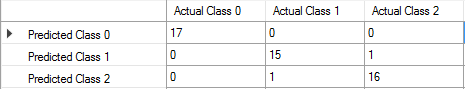
\includegraphics[width=\textwidth]{Iris_Test_CM.png}
\caption{Confusion Matrix}
\label{}
\end{figure}

Aus der Klasseneinteilung lässt sich die Genauigkeit bestimmen, welche hier 96\% beträgt. Der \textit{gini-index} daher ist 0,98 .

\subsection{Wisconsin Diagnostic Breast Cancer Datensatz}
Die Werte stammen aus einem digitalen Bild und beschreiben die Beschaffenheit der einzeln Zellen im Gewebe welche auf dem Bild zu sehen sind. \cite{uci}
\subsubsection{Eingabedaten}
\begin{itemize}
	\item Klassen: 2
	\item Datengröße: 569
\end{itemize}
\subsubsection{Parameter}
\begin{itemize}
	\item Train: 33\% Test: 67\%
	\item K: 3 
\end{itemize}
\subsubsection{Ergebnis}
\begin{figure}[H]
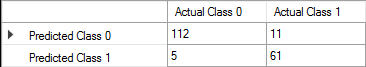
\includegraphics[width=\textwidth]{Cancer_Test_CM.png}
\caption{Confusion Matrix}
\end{figure}

Aus der Klasseneinteilung lässt sich die Genauigkeit bestimmen, welche hier 91.5\% beträgt. Der \textit{gini-index} daher ist 0,86 .

\subsection{Parkinsons Datensatz}
Der Datensatz stammt von 31 Personen, bei denen die Stimmen gemessenen worden sind, diesbezüglich hatten 23 die Krankheit Parkinson. \cite{uci}
\subsubsection{Eingabedaten}
\begin{itemize}
	\item Klassen: 2
	\item Datengröße: 195
\end{itemize}
\subsubsection{Parameter}
\begin{itemize}
	\item Train: 33\% Test: 67\%

	\item K: 7
\end{itemize}
\subsubsection{Ergebnis}
\begin{figure}[H]
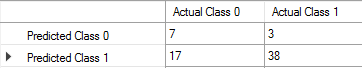
\includegraphics[width=\textwidth]{Parkinsons_Test_CM.png}
\caption{Confusion Matrix}
\end{figure}

Aus der Klasseneinteilung lässt sich die Genauigkeit bestimmen, welche hier 69.2\% beträgt. Der \textit{gini-index} ist daher 0,81.
\subsection{Fazit}
Aus den Ergebnissen kann ableitet werden, dass es bei der Klassifikation wichtig ist, das richtige Verhältnis zwischen Trainings- und Testdaten zu finden. Dies ist stark ausschlaggebend für die Qualität der Ergebnisse. Weiters ist auch zu beachten, dass das Verhältnis zwischen Datenreihen und Klassen entspricht, da sonst es zu Misklassifikationen kommen kann und dadurch zu einer Verschlechterung der Güte. Derzeitiger Stand ist, dass es keine wirkliche Regel für das Verhältnis zwischen Klassen und Anzahl der Daten gibt. Trotzdem sollte von einem relativ ausgeglichen Verhältnis ausgegangen werden.
\section{Clustering}
\subsection{Einführung}
Das Clustering wird anhand des \textit{k-means} Algorithmus gezeigt. Da ein Vergleich zwischen Clustering und Klassifikation erfolgen sollte, wurden herbei dieselben Datensätze verwendet. Der Unterschied zur Klassifikation ist, dass dabei die Klassendefinition weggelassen wird und stellt daher eine unüberwachte Klassifikation dar. Bei der Auswertung werden die Cluster gezeigt und die Zugehörigkeit gebildet. \cite{uci}
\subsection{Iris Datensatz}
\begin{itemize}
	\item Datengröße: 150
\end{itemize}
\subsubsection{Parameter}
\begin{itemize}
	\item K: 3 
	\item Wiederholungen: 0
\end{itemize}
\subsubsection{Ergebnis}
\begin{figure}[H]
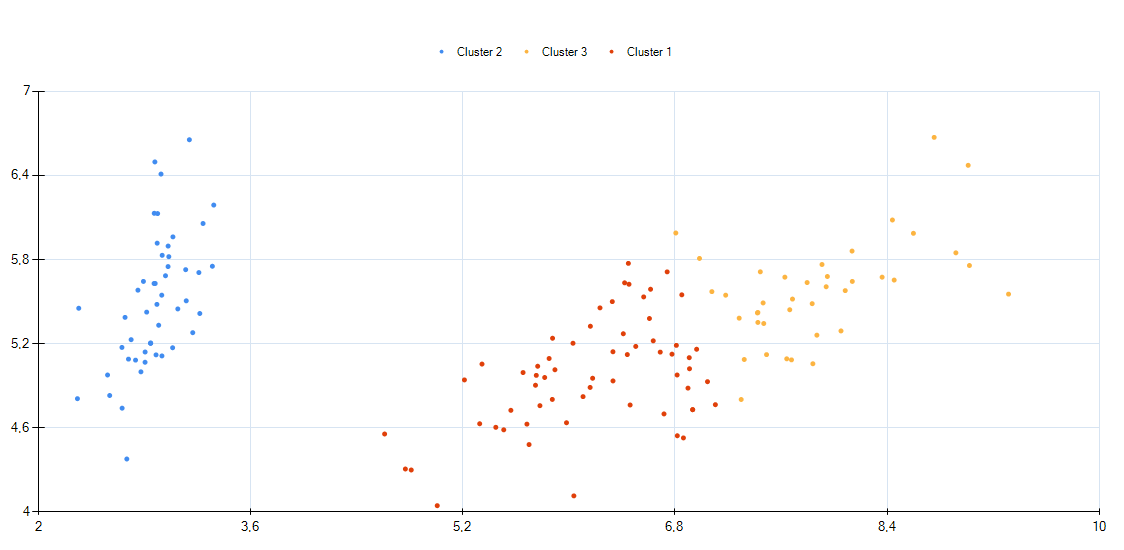
\includegraphics[width=\textwidth]{Iris_Test_CL.png}
\caption{Cluster}
\end{figure}

Wie zu erkennen ist gibt es wenige Ausreißer, da die Daten ursprünglich von einem Datensatz bezüglich Klassifikation stammen und bereits in Klassen dargestellt worden sind. 
\cite{uci}
\subsection{Wisconsin Diagnostic Breast Cancer Datensatz}
\begin{itemize}
	\item Datengröße: 569
\end{itemize}
\subsubsection{Parameter}
\begin{itemize}
	\item K: 3 
	\item Wiederholungen: 0
\end{itemize}
\subsubsection{Ergebnis}
\begin{figure}[H]
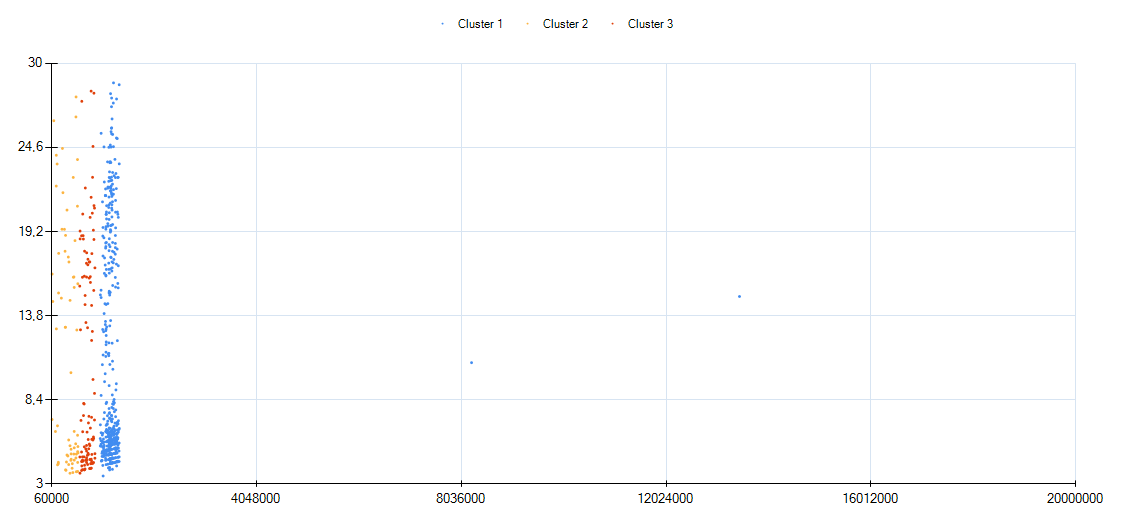
\includegraphics[width=\textwidth]{Cancer_Test_CL.png}
\caption{Cluster}
\end{figure}
Bei diesen Datensatz ist zu erkennen, dass es Ausreißer gibt,  diese werden trotzdem wegen der \textit{Ähnlichkeit} einiger Merkmale einem Cluster zugeordnet.
\cite{uci}
\subsection{Parkinsons Datensatz}
\begin{itemize}
	\item Datengröße: 195
\end{itemize}
\subsubsection{Parameter}
\begin{itemize}
	\item K: 2 
	\item Wiederholungen: 0
\end{itemize}
\subsubsection{Ergebnis}
\begin{figure}[H]
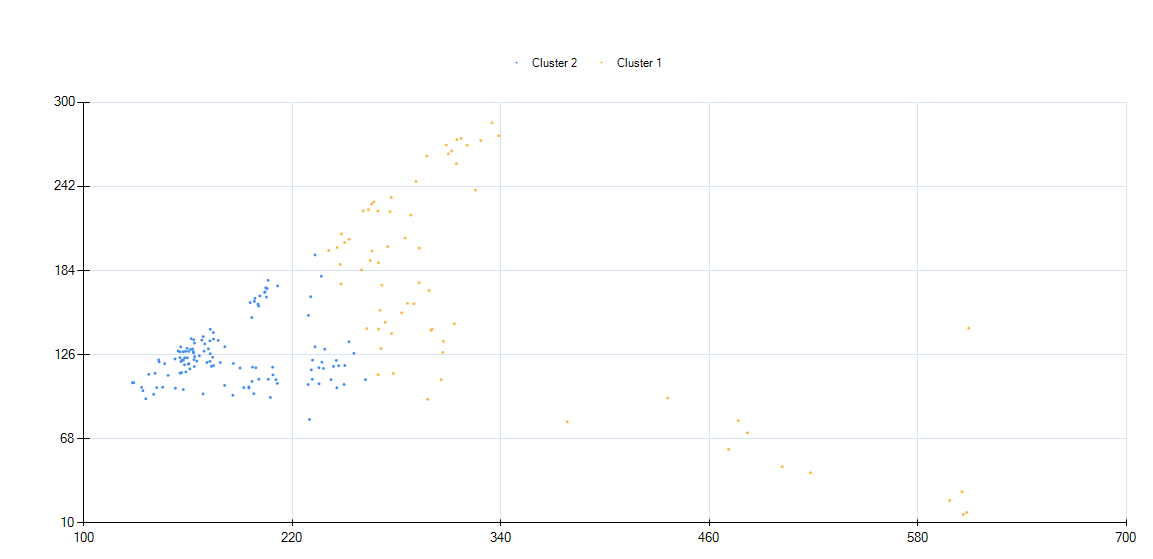
\includegraphics[width=\textwidth]{Parkinsons_Test_CL.png}
\caption{Cluster}
\end{figure}
Durch die Wahl von von zwei Clustern kann eine gute Klassifikation dargestellt werden, da die zwei vorgegeben Klassen relativ exakt dargestellt werden können 

\cite{uci}
\subsection{Fazit} 
Beim Clustering ist klar zu erkennen dass es Gemeinsamkeiten mit der Klassifikation gibt, da die meisten Clustereinteilungen die wahren Klassen voraussagen. Daher ist das Clustering ebenso bedeutend wie die Klassifikation. Beim Clustering kommt es auf die  vorgegebene Clusteranzahl an um gute Ergebnisse zu liefern.

\chapter{Schluss}
\section{Zusammenfassung}
In dieser Arbeit wurden die Themen Clustering und Klassifikation behandelt. Ziel war es die verschieden Algorithmen aufzuzeigen und zu vergleichen. Grundlegend wird von Klassifikation ausgegangen, die sich in eine überwachte und unüberwachte Klassifikation einteilen lässt. Bei der unüberwachten Klassifikation kann auch von Clustering gesprochen werden, da es hier keine eindeutige Klasseneinteilung gibt. Im Gegensatz dazu ist bei der klassischen Klassifikation die Einteilung bzw. die Zuordnung bekannt. Doch arbeiten beide Verfahren nach demselben Prinzip. Umfangreiche Daten werden in verwendbare Teile eingeteilt.\\
Die beiden Methoden spielen in der heutigen Welt eine große Rolle und werden häufig in der Datenanalyse sowie im Bereich des Data Mining verwendet. Daher sind unterschiedliche Algorithmen implementiert worden, um dieses Problem zu lösen. Dabei kommt es auf die verwendeten Daten an, welcher Algorithmus die besten Ergebnisse liefert.\\
Abschließend wird zusammengefasst, dass in dieser Arbeit nicht alle Algorithmen beschrieben worden sind. In dieser Arbeit wurden nur die bedeutsamsten und die relevanten Algorithmen aufgelistet. Die Algorithmen werden nicht nur für Clustering und Klassifikation verwendet, sondern auch in Bereichen wo Datenanalysen und Heuristiken eine wesentliche Rolle spielen.




\MakeBibliography
 
\end{document}
